\documentclass[11pt]{article}
\usepackage[margin=1in]{geometry}
\usepackage{graphicx}
\usepackage{amsmath}
% booktabs, hyperref, caption omitted so this compiles with a minimal TeX Live
% (e.g. Ubuntu: texlive-latex-base + texlive-latex-recommended). For prettier
% tables install: sudo apt install texlive-latex-extra

\title{Milestone Report: Learning to Select Density Functionals\\for GSCDB Reaction Energies}
\author{CS285 Project --- RL Functional Selector}
\date{\today}

\begin{document}
\maketitle

\begin{abstract}
We study the problem of choosing among a fixed set of density-functional approximations (DFAs) for predicting GSCDB reaction energies from molecular geometry alone. A neural policy is trained with supervised warm-start followed by batched REINFORCE, using pooled features from reactant and product \texttt{.xyz} files. On a held-out test split, the greedy policy achieves substantially lower mean absolute error (MAE) than choosing a functional uniformly at random, but remains well above an oracle that always picks the best DFA per reaction using tabulated energies. Training curves show rapid improvement during supervised pretraining and a plateau in classification-style metrics during the reinforcement-learning phase.
\end{abstract}

\section{Question and motivation}

Accurate reaction energies depend strongly on the choice of electronic-structure method. The Gold-Standard Chemical Database (GSCDB) provides reference reaction energies and tabulated values for many popular DFAs. The motivating question is:

\begin{quote}
\textit{Given only the geometries of the species involved in a reaction (reactants and products), can we predict which DFA will yield a reaction energy closest to the reference?}
\end{quote}

This is framed as a \emph{discrete decision problem}: the action space is the set of DFAs present in \texttt{Reaction\_Energies.csv}. Success is measured by (i) how often the model's top choice coincides with a lowest-error functional, and (ii) the MAE of the reaction energy for the predicted functional versus the reference.

\section{Method}

\subsection{Data and labels}
\begin{itemize}
  \item \textbf{Reactions:} Entries from \texttt{Info/DatasetEval.csv} are aligned with \texttt{Analysis/Reaction\_Energies.csv}. Stoichiometry strings are parsed so that negative stoichiometric coefficients correspond to \emph{reactants} and positive coefficients to \emph{products}, consistent with the database's energy-difference convention.
  \item \textbf{Geometry input:} For each species, features are extracted from \texttt{GSCDB/xyz\_files/<id>.xyz}: atom counts, coarse geometry statistics (e.g.\ radius of gyration, extrema of interatomic distances), and normalized element fractions. Reactant-side and product-side species are pooled (coefficient-weighted means) and concatenated with simple counts to form a fixed-length state vector per reaction.
  \item \textbf{Supervision signal:} For each reaction, the ``best'' functional index is the argmin of $|E_j - E_{\mathrm{ref}}|$ over DFAs $j$. Training rewards in REINFORCE use $r = -|E_{\hat j} - E_{\mathrm{ref}}|$ for the sampled action $\hat j$.
\end{itemize}

\subsection{Policy and training}
\begin{itemize}
  \item \textbf{Architecture:} A multi-layer perceptron with ReLU hidden layers outputs logits over DFAs; a softmax defines a stochastic policy $\pi(a \mid s)$.
  \item \textbf{Supervised warm-start:} Cross-entropy minimization toward the argmin-error label (batched SGD) provides a low-variance initial signal.
  \item \textbf{REINFORCE:} Batched policy-gradient updates with per-batch centered advantages reduce variance relative to single-sample updates. An entropy bonus encourages exploration. A moving average of batch-mean reward is logged as a training baseline (not a performance metric on the test set).
  \item \textbf{Evaluation split:} Reactions are shuffled; approximately 85\% train / 15\% test (typical run: $\sim$7{,}121 train / $\sim$1{,}256 test reactions when the full GSCDB subset with complete XYZ is used).
\end{itemize}

\subsection{Metrics}
\begin{itemize}
  \item \textbf{Test greedy accuracy:} Fraction of test reactions for which the greedy argmax functional achieves the minimum $|E - E_{\mathrm{ref}}|$ (ties count as correct).
  \item \textbf{Test MAE (greedy):} Mean over test reactions of $|E_{\hat a} - E_{\mathrm{ref}}|$ where $\hat a$ is the greedy action (Hartree).
  \item \textbf{Oracle MAE:} Mean over test reactions of $\min_j |E_j - E_{\mathrm{ref}}|$ --- the best achievable MAE if one always selected an optimal DFA from the tabulated list (uses energies at test time; not realizable from geometry alone).
  \item \textbf{Uniform-random MAE:} Monte Carlo estimate of the MAE when $j$ is drawn uniformly over DFAs (sanity baseline).
  \item \textbf{Probability on best:} Average total policy probability placed on all functionals tied for minimum error (smoother than greedy accuracy).
\end{itemize}

\section{Results}

\subsection{Representative numbers (one full training run)}
Table~\ref{tab:metrics} summarizes metrics consistent with logged training output: supervised warm-start improves greedy accuracy and MAE; after extended REINFORCE, greedy test accuracy can plateau while MAE remains between oracle and random baselines.

\begin{table}[htbp]
  \centering
  \caption{Illustrative test-set metrics (order of magnitude from a representative run with $\sim$1{,}256 test reactions and 16 DFAs).}
  \label{tab:metrics}
  \begin{tabular}{@{}lcc@{}}
    \hline
    Quantity & Value & Comment \\
    \hline
    Test greedy accuracy & $\sim 0.16$ & $\approx 16\%$ top-1 hits vs.\ $\sim 1/16 \approx 6\%$ random \\
    Test MAE (greedy) & $\sim 0.76$~Ha & $\sim 480$~kcal/mol \\
    Oracle MAE & $\sim 0.19$~Ha & Lower bound among listed DFAs \\
    Uniform-random MAE & $\sim 1.7$~Ha & Weak baseline \\
    \hline
  \end{tabular}
\end{table}

The model clearly \textbf{beats random selection} on MAE but is \textbf{far from oracle}: simple geometry descriptors do not fully determine which functional wins across diverse GSCDB sets.

\subsection{Training dynamics (figures)}
Figure~\ref{fig:overview} shows four panels over cumulative updates (warmup indices $1\ldots W$, then REINFORCE $W{+}1, \ldots$). \textbf{Top-left:} test and train greedy accuracy rise during supervised warmup; the vertical line marks the switch to REINFORCE. \textbf{Top-right:} test MAE in Hartree with oracle (green) and random (orange) reference lines --- the learned curve should lie between them when the policy is informative. \textbf{Bottom-left:} probability mass on truly best functionals. \textbf{Bottom-right:} REINFORCE reward baseline (training diagnostic).

\begin{figure}[htbp]
  \centering
  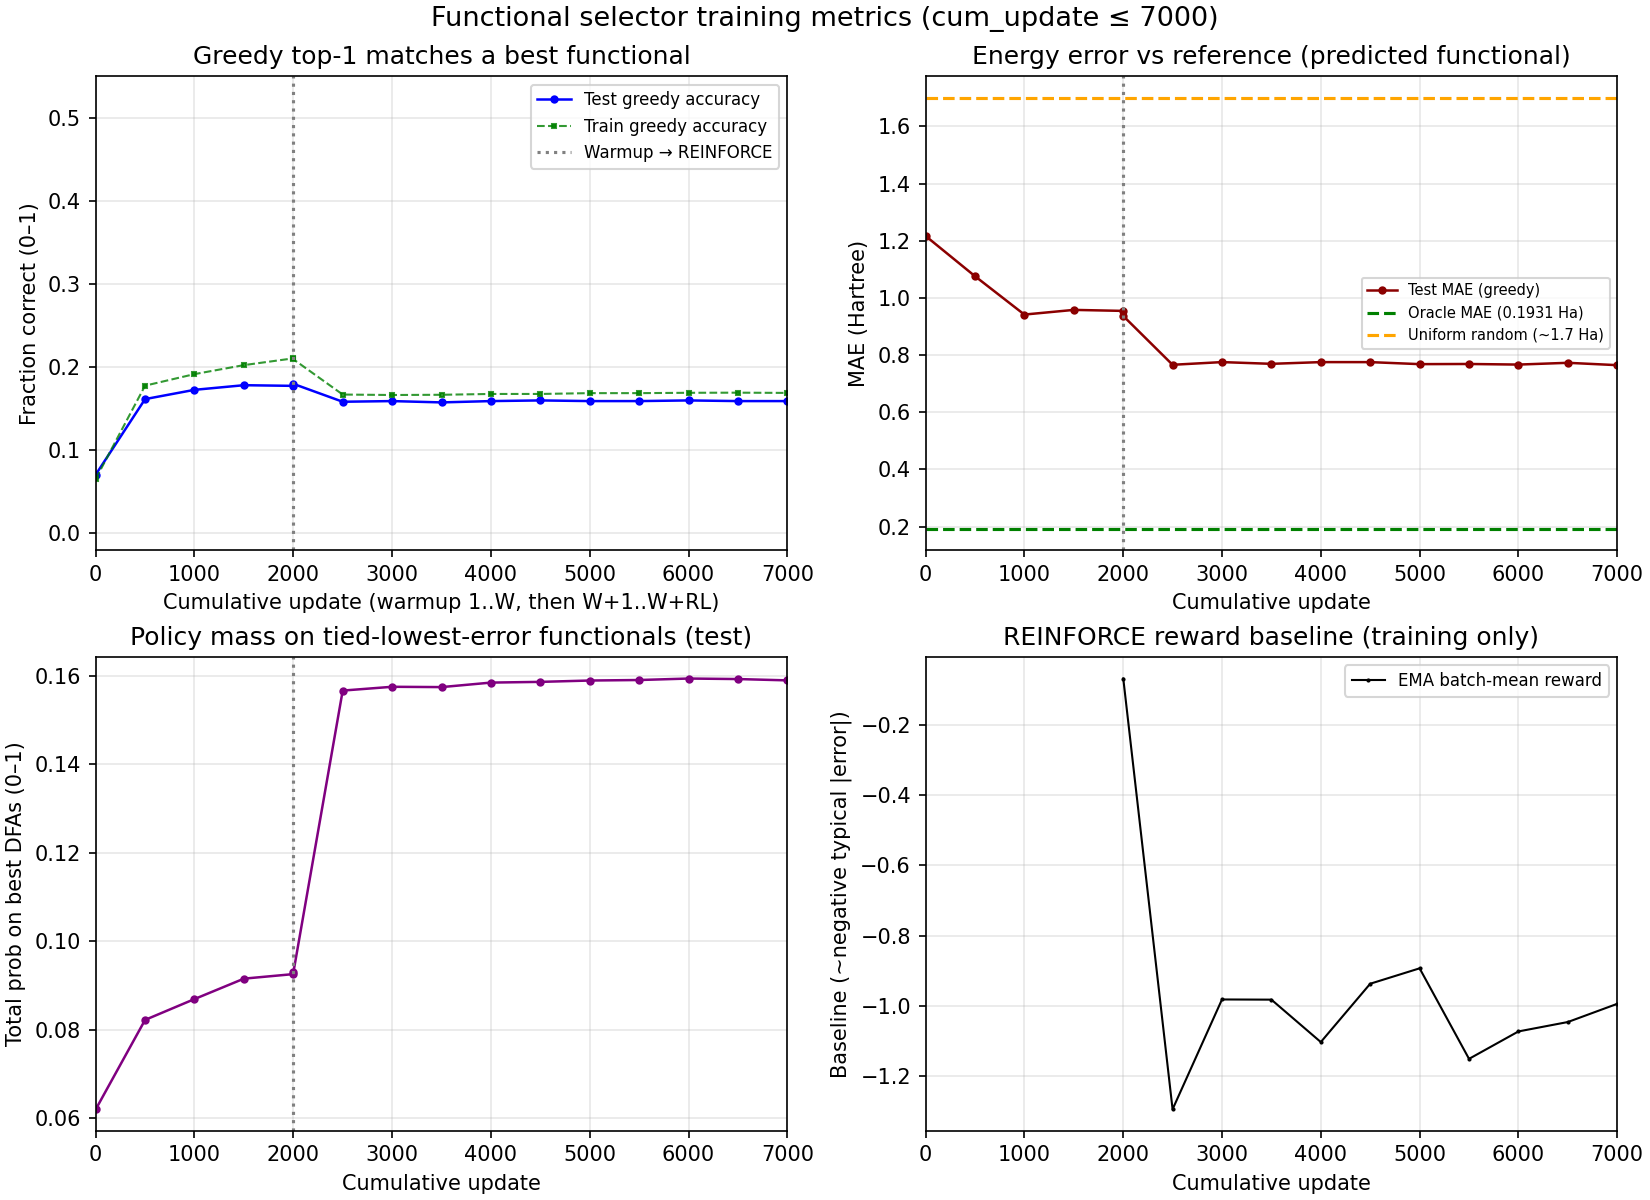
\includegraphics[width=\textwidth]{models/reaction_reinforce/plots/training_curves_overview_first7000.png}
  \caption{Training metrics for the first 7000 cumulative logged updates (warmup + early REINFORCE).}
  \label{fig:overview}
\end{figure}

Figure~\ref{fig:maekcal} plots the same test MAE in kcal/mol for interpretability (1~Hartree $\approx 627.5$~kcal/mol).

\begin{figure}[htbp]
  \centering
  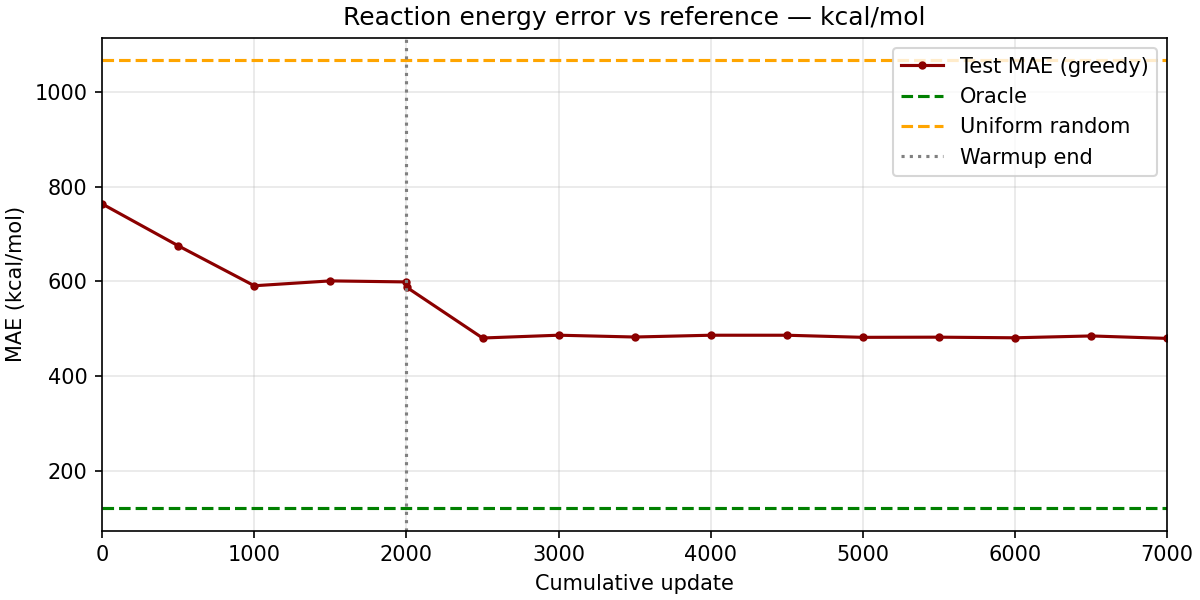
\includegraphics[width=0.85\textwidth]{models/reaction_reinforce/plots/training_mae_kcal_mol_first7000.png}
  \caption{Test MAE versus reference in kcal/mol (first 7000 cumulative updates).}
  \label{fig:maekcal}
\end{figure}

\section{Discussion}
Greedy accuracy is a \emph{hard} metric: small logit changes rarely flip the argmax, so curves can appear flat even while MAE or probability-on-best move. REINFORCE optimizes expected sampled reward, not greedy test accuracy, which can explain post-warmup regressions or plateaus in top-1 accuracy. The gap to oracle indicates that stronger representations (e.g.\ dataset identity, richer descriptors, or graph-based models) would likely be needed for large gains.

\section{Next steps}
\begin{itemize}
  \item Extend the state with dataset identifiers or stoichiometry metadata.
  \item Train primarily with supervised or soft-label objectives aligned with MAE or ranking.
  \item Report confidence intervals over multiple random seeds and splits.
\end{itemize}

\paragraph{Reproducibility.}
Train: \texttt{python train\_reaction\_reinforce.py --gscdb-root ../../GSCDB --out-dir ../models/reaction\_reinforce}. Plots: \texttt{python plot\_training\_curves.py --history ../models/reaction\_reinforce/training\_history.json --max-cum-update 7000}. Compile this document from the \texttt{RL\_Functional\_Selector} directory so figure paths resolve.

\end{document}
